\section[Обзор технологий организационного управления]{%
  ОБЗОР ТЕХНОЛОГИЙ ОРГАНИЗАЦИОННОГО \\
  УПРАВЛЕНИЯ
}
\label{sec:org_management}

Поскольку компания занимается разработкой программного обеспечения,
логично предположить, что рабочий процесс каждого отдельного сотрудника компании
автоматизирован в полной мере.

Рабочее место сотрудника компании оснащено персональным компьютером. 
Персональные компьютеры сотрудников подключены к единой сети, являющейся
универсальным средством обмена информацией в рамках системы.
Сеть позволяет передавать между компьютерами любые данные --- 
документы, изображения, звук и другие файлы, предоставляя удобные возможности
для коммуникации между сотрудниками предприятия, между структурными подразделениями 
и между предприятием и клиентом. 

Основным средством для деловой коммуникации в компании является электронная почта.
Преимущества электронной почты:
\begin{itemize}
\item быстрая доставка сообщений; 
\item возможность переписки с несколькими адресатами;
\item достаточная степень формализованности обмена сообщениями,
  позволяющая вести полноценную деловую переписку c заказчиком.
\end{itemize}

Для оперативного общения используются приложения Skype и Lync,
предоставляющие возможность общения в реальном режиме времени 
посредством текстовых сообщений, а также аудио и видео.

Системы корпоративного планирования и управления являются одной из
важнейших составляющих информационной структуры современного предприятия.
Такие системы предоставляют методы планирования и использования ресурсов предприятия, 
управление взаимоотношениями с клиентами, а также моделирование логистической цепи поставок.
Это ускоряет бизнес-процессы на предприятии, позволяя ему более эффективно реагировать на
изменения среды, действовать в рамках концепции производства, ориентированного на клиента,
внедрить систему централизованного управления качеством.

Рассмотрим составляющие части системы корпоративного управления 
компании EPAM Systems.

\newpage

\textbf{EPAM information portal} представляет собой каталог внутренних ресурсов EPAM.
Этот ресурс представляет собой единую точку входа во все внутренние корпоративные ресурсы
компании.

Интерфейс EPAM information portal представлен на рисунке~\ref{pic:epam_info}.

\begin{figure}[h!]
  \centering
  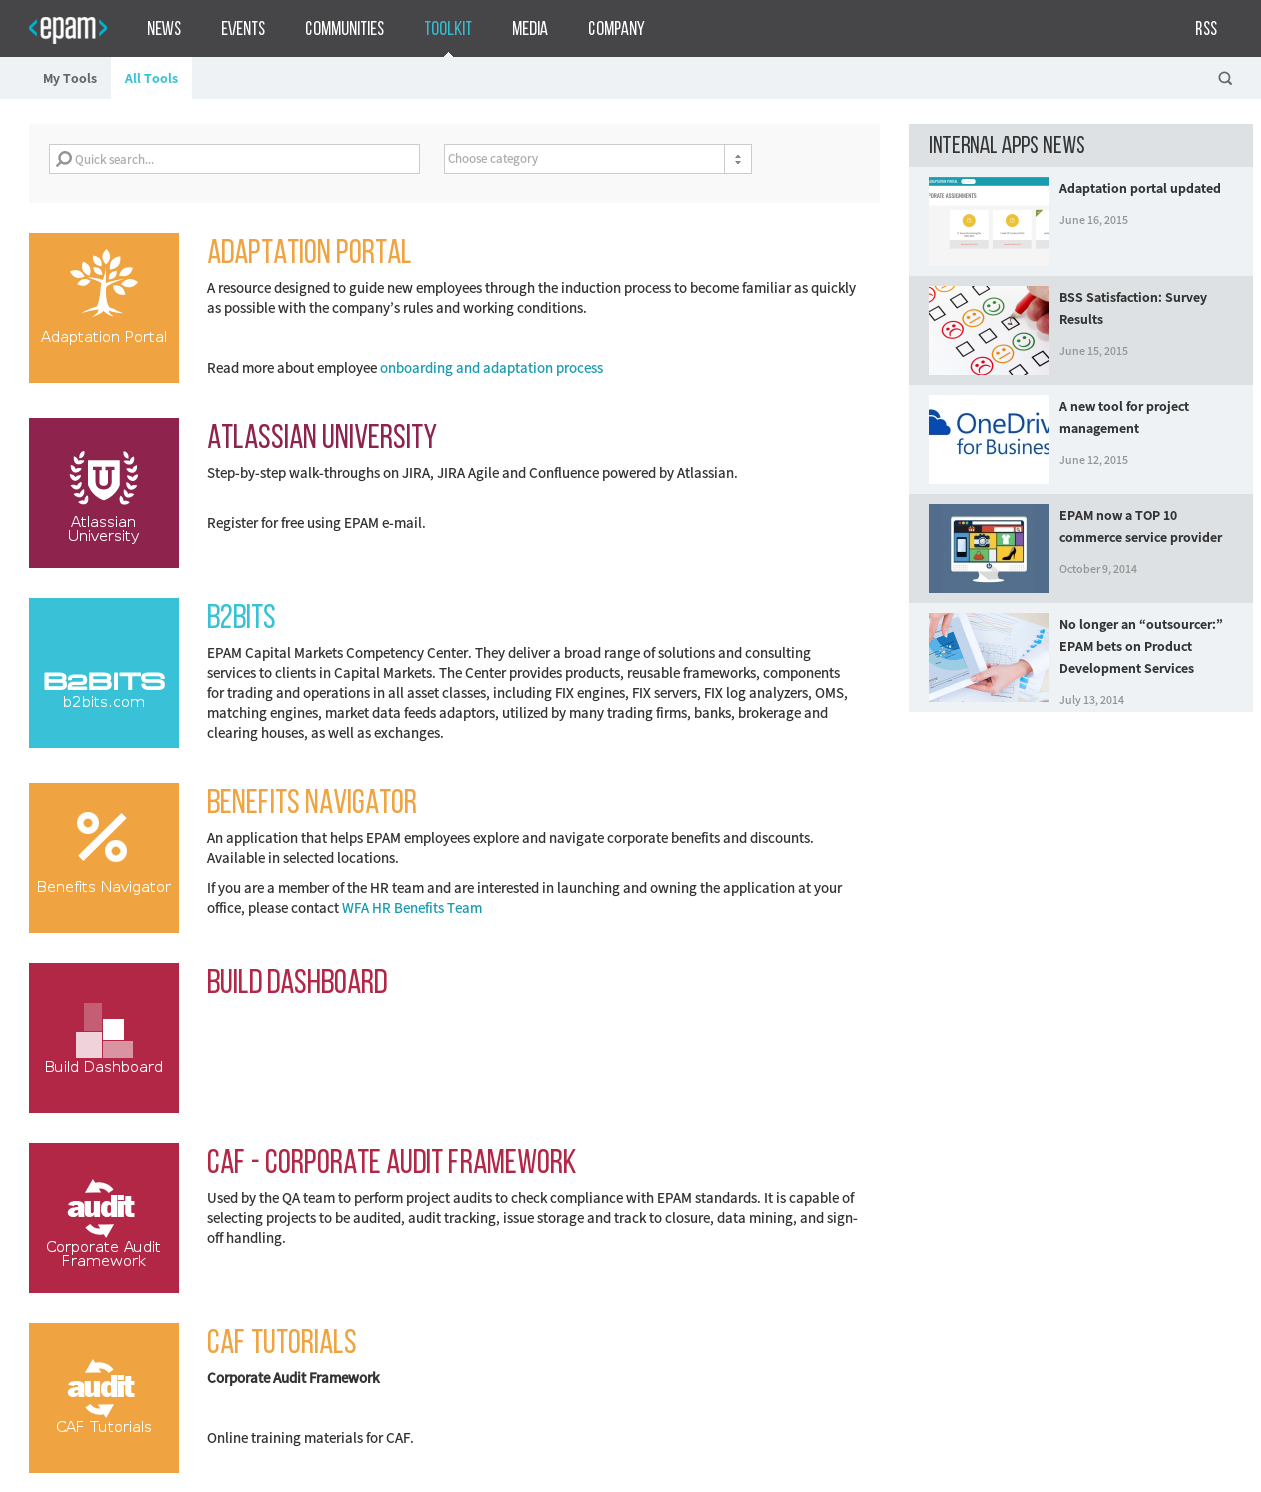
\includegraphics[width=150mm]{pic/epam_info.png}
  \caption{Использование EPAM information portal}
  \label{pic:epam_info}
\end{figure}

\newpage

\textbf{EPAM adaptation portal} представляет собой сервис, предназначенный для
облегчения адаптации новых сотрудников EPAM. 
Этот ресурс предоставляет информацию о процедурах оформления, 
организации контроля качества, обзоры бизнес-процессов,
проектной документации и бенефитов, предоставляемых сотрудникам компании.

Интерфейс EPAM adaptation portal представлен на рисунке~\ref{pic:epam_adaptation}.

\begin{figure}[h!]
  \centering
  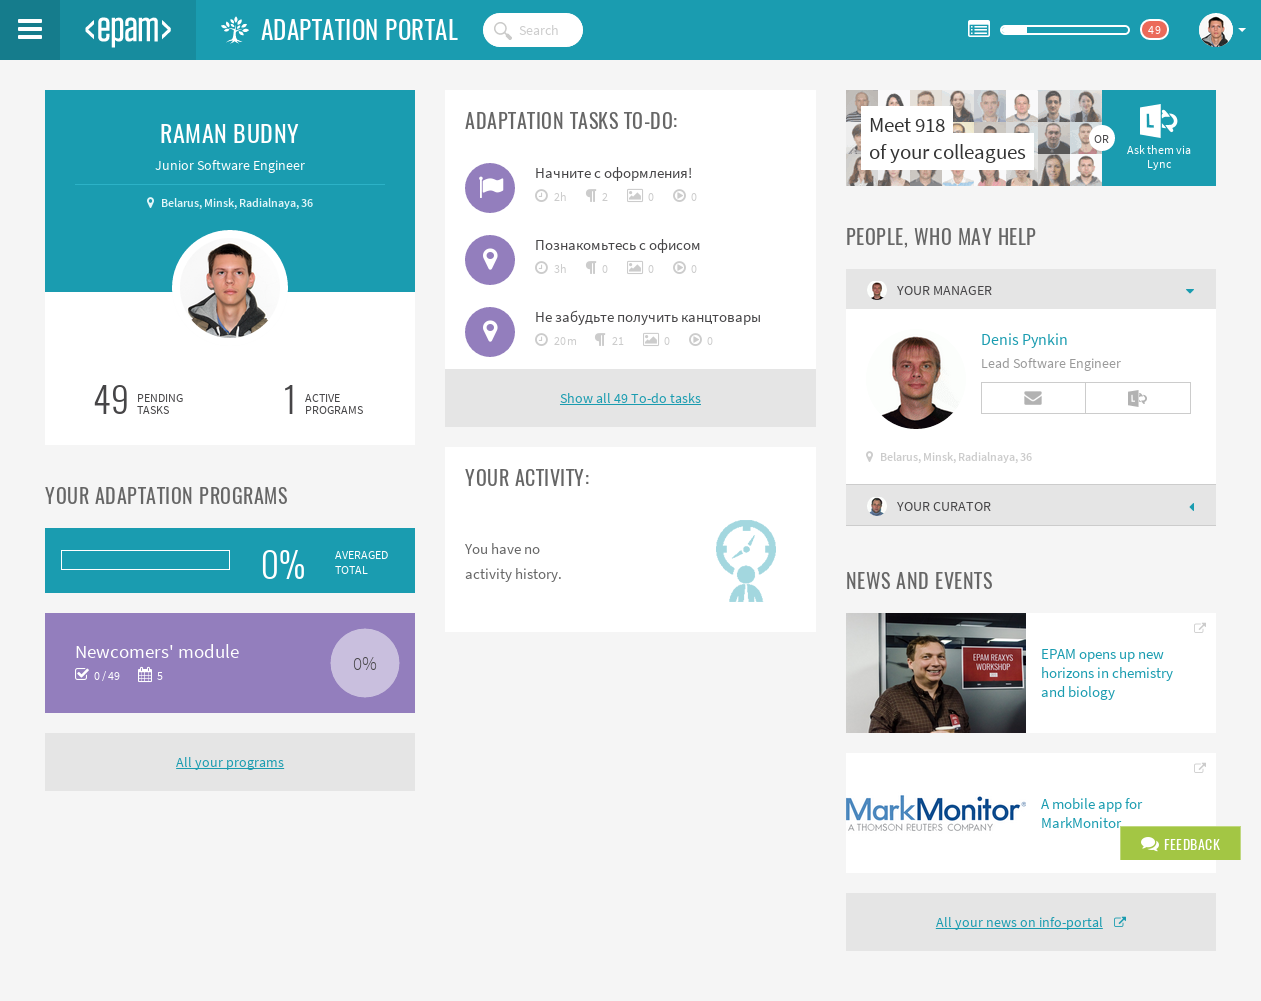
\includegraphics[width=150mm]{pic/epam_adaptation.png}
  \caption{Использование EPAM adaptation portal}
  \label{pic:epam_adaptation}
\end{figure}

\newpage

\textbf{EPAM employee handbook} --- сервис, предоставляющий наиболее актуальную
информацию о различных сферах деятельности работников компании:
\begin{itemize}
\item политика коммуникации с заказчиками;
\item политика безопасности;
\item политика качества;
\item образовательные программы;
\item перспективы карьерного роста;
\item возможности, предоставляемые офисом;
\item организация беспроводного доступа в интернет;
\item элементы корпоративного дизайна;
\item бенефиты, предоставляемые сотрудникам.
\end{itemize}


Интерфейс EPAM emloyee handbook представлен на рисунке~\ref{pic:epam_handbook}.

\begin{figure}[h!]
  \centering
  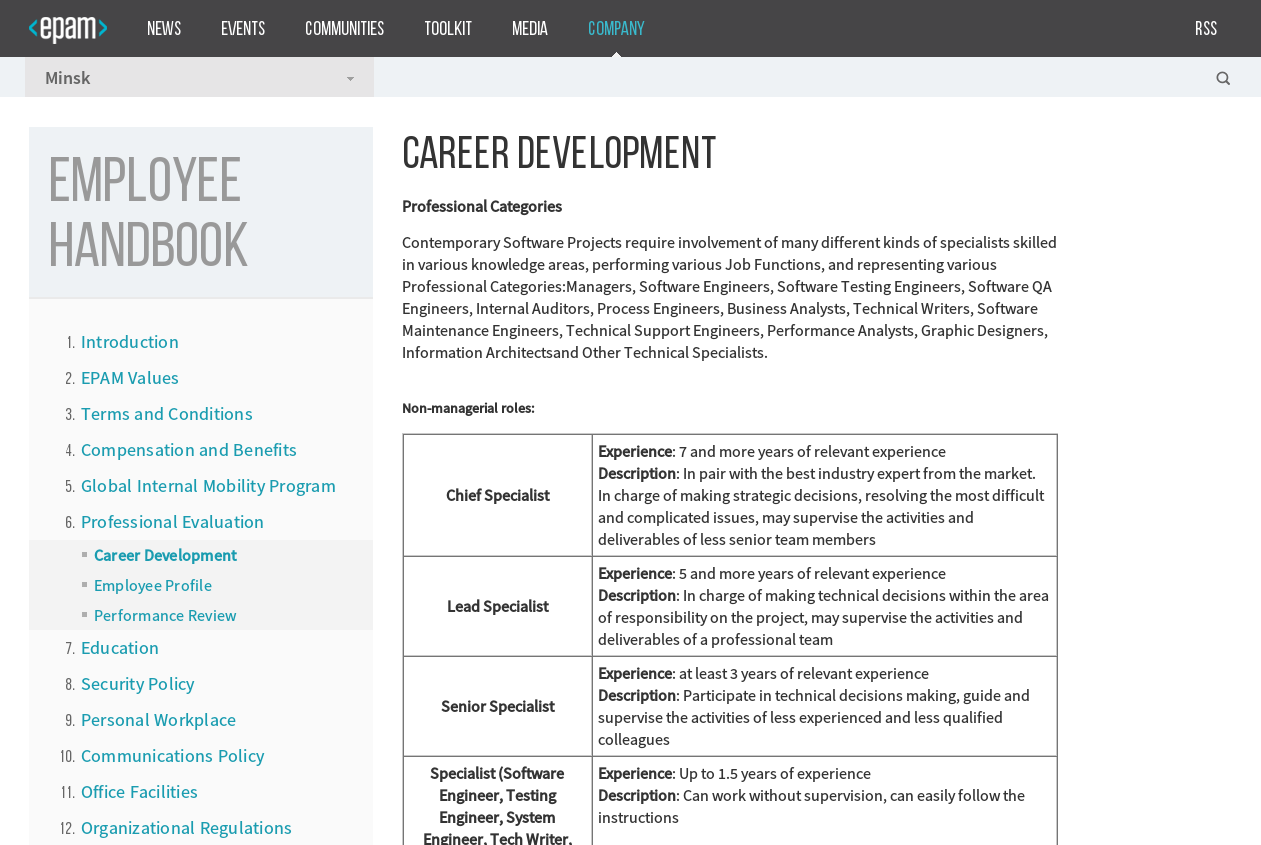
\includegraphics[width=150mm]{pic/epam_handbook.png}
  \caption{Использование EPAM employee handbook}
  \label{pic:epam_handbook}
\end{figure}

\newpage


\textbf{EPAM project management center} (PMC) представляет собой веб-ориентированную среду
для управления проектами. 
Функции EPAM PMC:
\begin{itemize}
\item обеспечение планирования проектов;
\item управление рисками и требованиями проекта;
\item контроль за выполнением проектных и ресурсных планов.
\end{itemize}

Интерфейс EPAM PMC представлен на рисунке~\ref{pic:epam_pmc}.

\begin{figure}[h!]
  \centering
  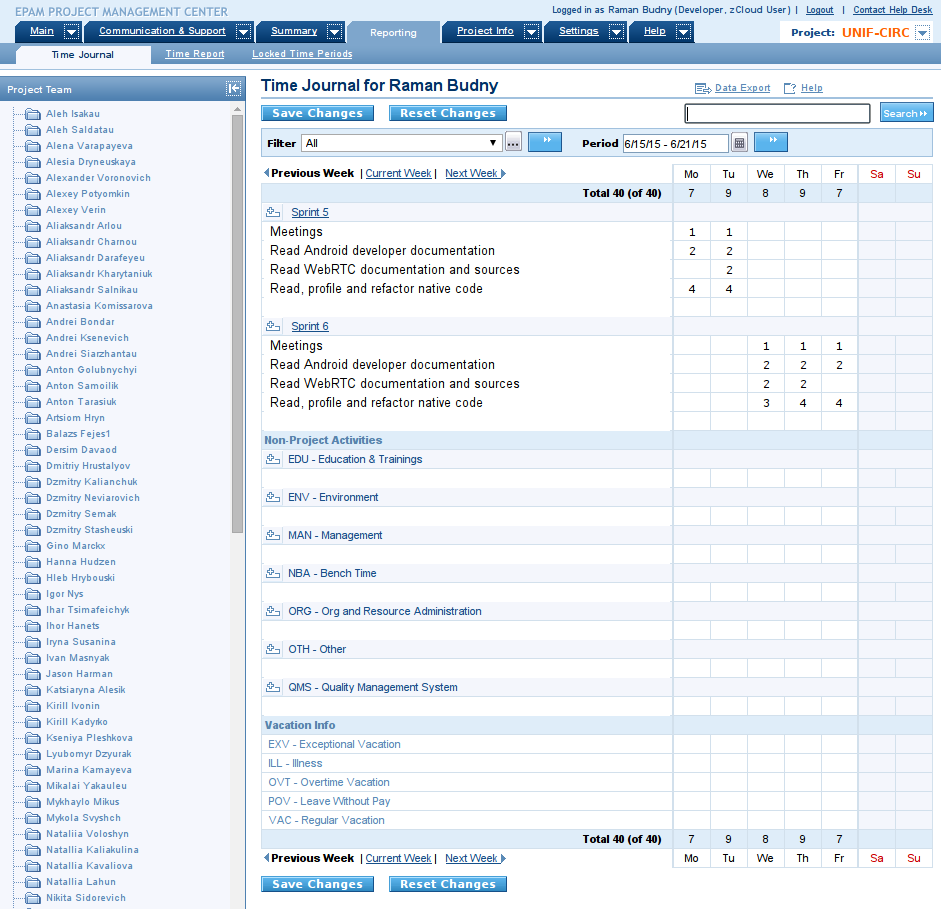
\includegraphics[width=150mm]{pic/epam_pmc.png}
  \caption{Использование EPAM PMC}
  \label{pic:epam_pmc}
\end{figure}

\newpage

\textbf{EPAM utilization and project staffing analyzer} (UPSA) представляет собой
автоматизированную среду для выполнения задач, связанных с управлением персоналом компании,
создания необходимых условий для привлечения новых людей, планирования загрузки персонала на проектах.

UPSA обладает следующими возможностями:
\begin{itemize}
\item осуществление проектного планирования в части управления человеческими ресурсами;
\item анализ и управление рабочей нагрузкой сотрудников компании;
\item оценка сотрудников проектных команд;
\item расширенный поиск и фильтрация сотрудников и проектов;
\item наличие средств для построения отчетов.
\end{itemize}

Интерфейс EPAM UPSA представлен на рисунке~\ref{pic:epam_upsa}.

\begin{figure}[h!]
  \centering
  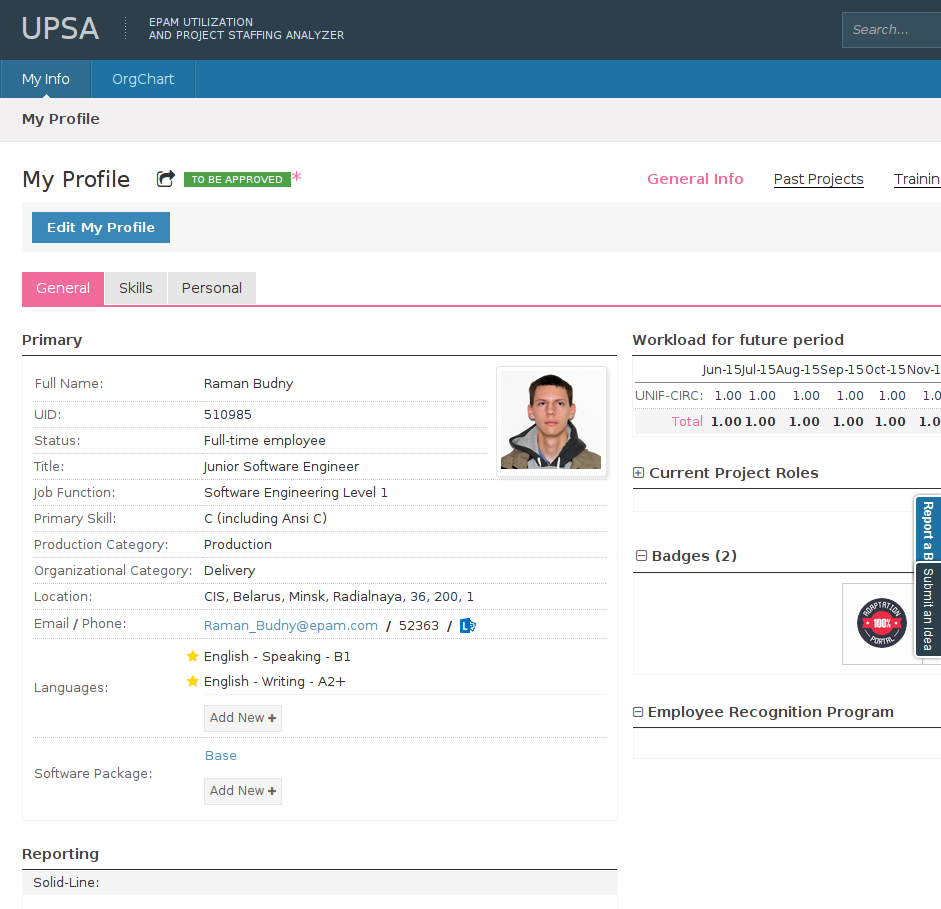
\includegraphics[width=150mm]{pic/epam_upsa.png}
  \caption{Профиль работника EPAM в UPSA}
  \label{pic:epam_upsa}
\end{figure}
